%\tableofcontents
\newpage

{\centering
\section{Introduzione all'apparato sperimentale}
}
\medskip
{\color{gray}\hrule}
\medskip


La prima parte dell’esperienza consiste nell’allineamento ottico del sistema di misura: definire con precisione l’asse ottico assicura infatti che il fascio luminoso attraversi coassialmente tutte le componenti dell’apparato, condizione necessaria per ottenere le frange di interferenza circolari e concentriche per l'osservazione dell’effetto Zeeman.

Il banco ottico è costituito da una rotaia su cui vengono montati, lungo l’asse ottico, un diaframma a iride, una lente convergente, un interferometro di Fabry-Perot, un'altra lente convergente, una lamina a quarto d'onda, un polarizzatore lineare e una ultima lente convergente
(si veda la figura \ref{fig:banco}).
A un’estremità della rotaia è posta una telecamera CCD, connessa a un software di acquisizione immagini, mentre sull’altra estremità è collocato un magnete a doppia bobina (883 spire per ciascuna bobina) con espansioni polari estraibili e forate, tra le quali viene inserita, quando necessario, la lampada spettrale ai vapori di Cadmio.
Un filtro spettrale rosso viene collocato lungo il cammino ottico per selezionare, tra tutte le righe spettrali del Cadmio, quella di interesse, corrispondente alla transizione atomica $3^1D_2 \rightarrow 2^1P_1$, sulla quale si vuole osservare l’effetto Zeeman.
\begin{figure}[H]
    \centering
    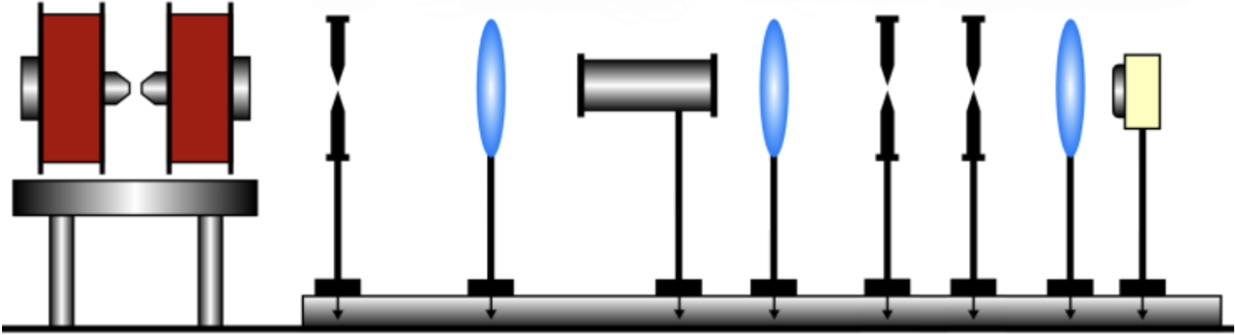
\includegraphics[width=0.8\linewidth]{banco.jpeg}
    \caption{\footnotesize Schema del banco ottico con magnete in configurazione longitudinale.}
    \label{fig:banco}
\end{figure}
Per l’allineamento del sistema ottico si utilizza un laser a bassa potenza, che consente di definire e verificare l’asse ottico dell’apparato, cosicchè
%testo di magda
una volta accesa la lampada spettrale, il sistema di acquisizione mostra una serie di anelli concentrici, ciascuno dei quali corrisponde a un diverso ordine di interferenza e, per una data lunghezza d’onda, a un angolo di emissione specifico.

Le diverse componenti spettrali della radiazione emessa dalla lampada generano quindi gruppi di anelli tra loro leggermente separati, la cui posizione radiale dipende dalla lunghezza d’onda della radiazione.
Sono proprio queste le frange che verranno utilizzate per misurare la separazione delle righe spettrali indotta dell'effetto Zeeman.
\newpage